\section{Introduction}

Many Bayesian inference problems such as preference
learning~\cite{sanner:aistats10} or trader valuation modeling in
financial markets naturally use piecewise
likelihoods~\cite{Shogren:00}, e.g., preferences may induce
constraints on possible utility functions while trader transactions
constrain possible instrument valuations.  To be concrete, consider
the following Bayesian approach to preference learning where our
objective is to learn a user's weighting of attributes for
classes of items (e.g., cars, apartment rentals, movies) given their
responses to pairwise comparison queries over those items:

%%%%%%%%%%%%%%%%%%%%%%%%%
\begin{figure*}%[t!]
%\centering
%\begin{subfigure}{.2\textwidth}
%  \centering
%  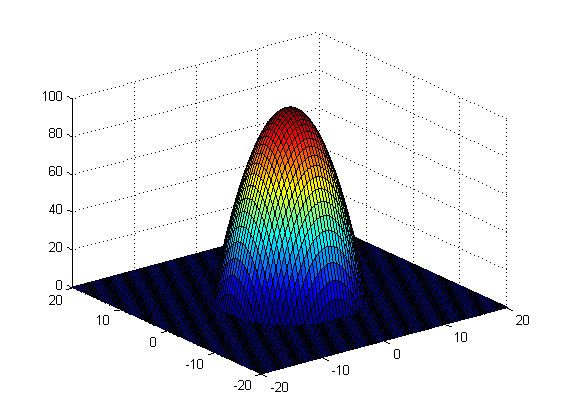
\includegraphics[width=.99\textwidth]{pic/bpplPriorII.png}
%  \label{fig:prior2d}
%\end{subfigure}%
\begin{subfigure}{.24\textwidth}
\centering
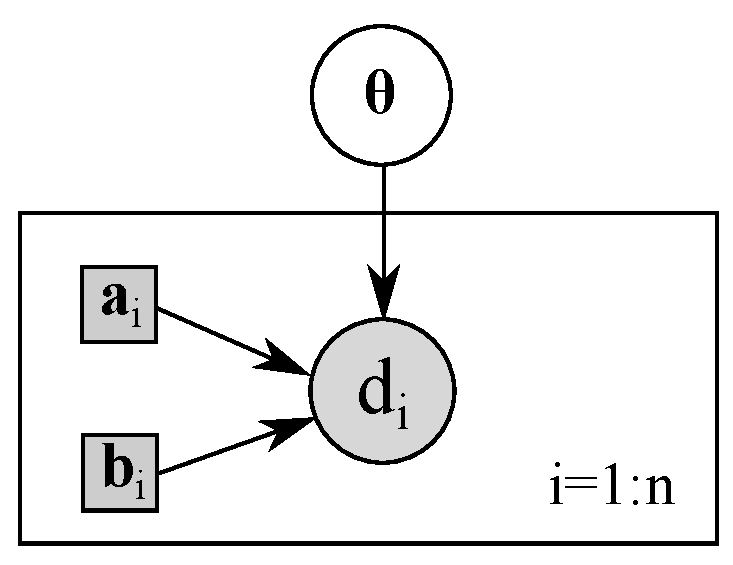
\includegraphics[width=1.0\textwidth]{pic/pref2w.pdf}
\end{subfigure}
%\begin{subfigure}{.2\textwidth}
%  \centering
%  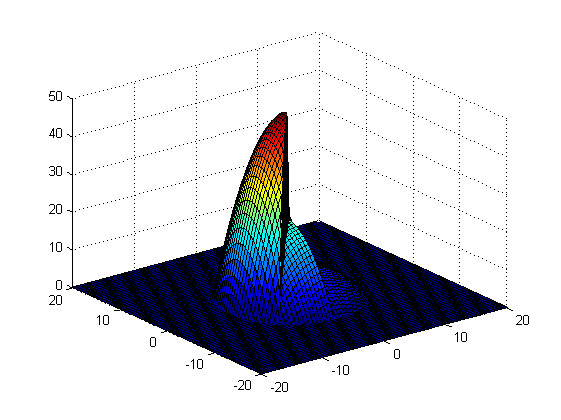
\includegraphics[width=.99\textwidth]{pic/bpplPosteriorII.png}
%  \label{fig:prior2d}
%\end{subfigure}%
%\label{fig:pref}
%\end{figure}
%%%%%%%%%%%%%%%%%%%%%%%%%
%\begin{figure}%[t!]
%\centering
%\begin{subfigure}{.2\textwidth}
%  \centering
%  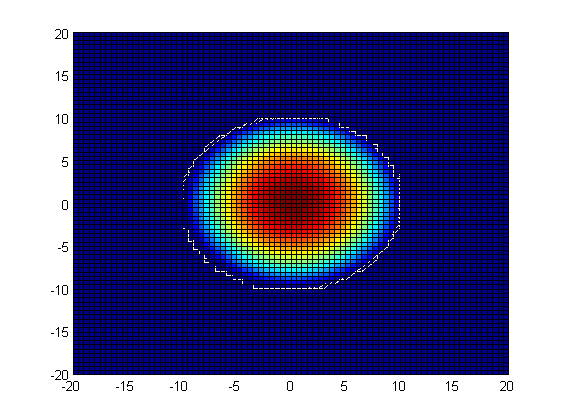
\includegraphics[width=.99\textwidth]{pic/bpplPriorART.png}
%  \label{fig:prior2d}
%\end{subfigure}%
\begin{subfigure}{.76\textwidth}
\centering
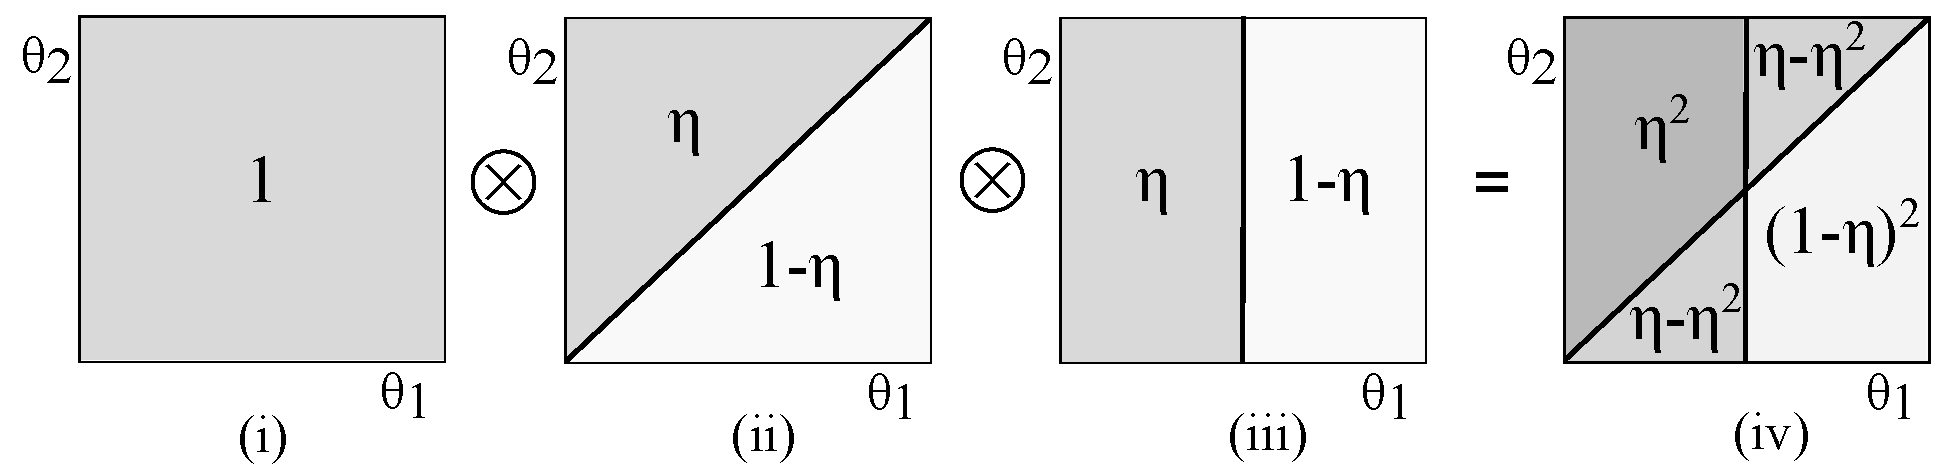
\includegraphics[width=1.0\textwidth]{pic/running1.pdf}
\label{fig:pref}
\end{subfigure}
%\begin{subfigure}{.2\textwidth}
%  \centering
%  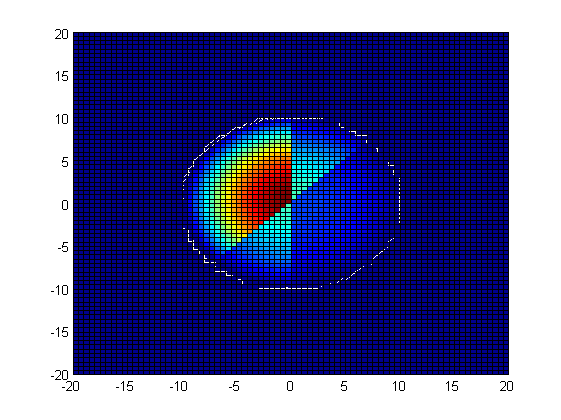
\includegraphics[width=.99\textwidth]{pic/bpplPosteriorIII.png}
%  \label{fig:prior2d}
%\end{subfigure}%
\caption{\footnotesize 
(a) Graphical model for BPPL problem in Example \ref{example:pref}.
(b) A 2D instance of Example \ref{example:pref}: 
(i) An (unnormalized) prior uniform in a rectangle with center (0,0).
(ii) Likelihood model $pr(\bvec{a}_1 \succ \bvec{b}_1 | \, \boldsymbol\theta)$ and
(iii) $pr(\bvec{a}_2 \succ \bvec{b}_2 | \, \boldsymbol\theta)$ 
(as in equation~\ref{e:pref1likelihood}) where
$\bvec{a}_1 = (5, 3)$, $\bvec{b}_1 = (6, 2)$, $\bvec{a}_2 = \bvec{a}_1$ and $\bvec{b}_2 = (6, 3)$.
(iv) A piecewise function proportional to the posterior distribution.}
\label{fig:pref-up-down}
%\caption{\footnotesize Graphical model for BPPL problem in Example \ref{example:pref}. }
\end{figure*}
% \vspace{2mm}
%%%%%%%%%%%%%%%%%%%%%%%%%
\fexample{example:pref}{Bayesian pairwise preference learning (BPPL)}{
  Suppose each \emph{item} $\bvec{a}$ is modeled by an $N$-dimensional
  real-valued \emph{attribute choice vector} $(\alpha_1, \ldots,
  \alpha_N)$.  The goal is to learn an \emph{attribute weight vector}
  $\boldsymbol\theta = (\theta_1, \ldots, \theta_N) \in \mathbb{R}^N$
  that describes the utility of each attribute choice from user
  responses to preference queries.  As commonly done in
  \emph{multi-attribute utility theory} \cite{Keeney:93}, the overall
  item utility $u(\bvec{a}|\, \boldsymbol\theta)$ is decomposed 
  additively over the attribute choices of $\bvec{a}$:
%
$$
u(\bvec{a} | \, \boldsymbol\theta) = \sum_{j=1}^N \theta_j\cdot\alpha_j
$$
%
User responses are in the form of $n$ queries (i.e.\ observed data
points) $d_1$ to $d_n$ where $d_i$ is a pairwise comparison of some
items $\bvec{a}_i$ and $\bvec{b}_i$ with the following possible
responses:
\begin{itemize}\denselist
\item $\bvec{a}_i \succ \bvec{b}_i$:  In the $i$-th query, the user prefers item $\bvec{a}_i$ over $\bvec{b}_i$.
\item $\bvec{a}_i \preceq \bvec{b}_i$:  In the $i$-th query, the user does not prefer item $\bvec{a}_i$ over $\bvec{b}_i$.
\end{itemize}
It is assumed that with an \emph{elicitation noise} $0 \leq \eta <
0.5$, the item with a greater utility is preferred:
\begin{align}
\label{e:pref1likelihood}
pr(\bvec{a}_i \succ \bvec{b}_i \,|\, \boldsymbol\theta) =
{\footnotesize
\begin{cases}
u(\bvec{a}_i|\boldsymbol\theta) < u(\bvec{b}_i|\boldsymbol\theta) : \eta\\
u(\bvec{a}_i|\boldsymbol\theta) = u(\bvec{b}_i|\boldsymbol\theta) : 0.5\\
u(\bvec{a}_i|\boldsymbol\theta) > u(\bvec{b}_i|\boldsymbol\theta) : 1-\eta
\end{cases}
}%end footnote size
\\
pr(\bvec{a}_i \preceq \bvec{b}_i \,|\, \boldsymbol\theta) = 
1 - pr(\bvec{a}_i \succ \bvec{b}_i \,|\, \boldsymbol\theta)
\end{align}
As the graphical model in Figure~\ref{fig:pref-up-down} illustrates, our posterior
belief over the user's attribute weights is provided by the standard
Bayesian inference expression:
$
pr(\boldsymbol\theta | \, d_1, \ldots, d_n) 
\propto pr(\boldsymbol\theta) \cdot \prod_{i=1}^{n} pr(d_i | \, \boldsymbol\theta)
$. As also evidenced, since the
prior and likelihoods are piecewise distribitions, the posterior
distribution is also piecewise.  
} %end example 1
\vspace{2mm}
%%%%%%%%%%%%%%%%%%%%%%%%%%%%%%%%%%%%%%%%

Unfortunately, Bayesian inference in models with piecewise likelihoods
like BPPL in Example~\ref{example:pref} often lead to posterior
distributions with a number of piecewise partitions \emph{exponential in the
number of data points and attributes}, thus rendering exact analytical inference impossible.
While (Markov Chain) Monte Carlo methods provide an attractive
asymptotically unbiased approximation approach, rejection sampling and
Metropolis-Hastings both prove inefficient in practice, and analytical
derivation of Gibbs samplers require exponential space and time in the
number of data points and attributes of data.

%However, the number of partitions in
%the posterior grow exponential as the amount of observed data grows.
%In the following it will be shown that such a complexity not only
%prohibits exact inference to be carried out on piecewise modes with
%large number of observed points, but also the speed and convergence
%rate of asymptotically unbiased methods can be negatively affected.
%Based on our experiments, in particular, the speed of \emph{Gibbs
%  sampling} (and to a lesser extend, \emph{rejection sampling})
%rapidly decreased as the number of observed data points increase.  In
%this paper, we will present a variation of Gibbs sampling with an
%exponential-to-linear reductions in the amount of computations
%performed in each sampling step.

In this work, we show how to transform problematic
piecewise likelihoods into equivalent mixture models and provide
a blocked Gibbs sampling approach for this transformed model that
achieves an \emph{exponential-to-linear} reduction in space and time compared
to a conventional Gibbs sampler.  This enables fast, asymptotically
unbiased Bayesian inference in a new expressive class of piecewise graphical
models and empirically requires orders of magnitude less time than
rejection, Metropolis-Hastings, and conventional Gibbs sampling
methods to achieve the same level of accuracy -- especially
when the number of posterior partitions grows rapidly in the number of observed data points.

%Many real world Bayesian inference problems such as preference
%learning, predicting traders’ behavior in a financial market,
%competitive skill learning, etc. naturally have piecewise likelihood
%and/or prior models. To date tools for carrying out Bayesian reasoning
%in such models are either approximate (namely, approximate message
%passing with Gaussian priors/posteriors) or unscalable. The latter
%group consists of sampling-based methods limited to
%Metropolis-Hastings and rejection sampling. They are considered
%unscalable since in many models their convergence rate is slow (in
%time).  For the algorithms that require tuning, this is particularly
%true if they are not tuned well.  In practice, such a tunning can be
%difficult and problem-dependent.
%
%Gibbs sampling, does not require any tuning.  Nonetheless, when
%applied to piecewise models, its time/space computation costs can grow
%exponential in the amount of observed data.  This is prohibitively
%expensive and to our knowledge, so far, Gibbs sampling has not been
%used in the aforementioned models.

%Our work fills this gap by providing a Bayesian inference method which
%is both scalable and asymptotically unbiased that can be used in a
%large family of piecewise Bayesian models.  In particular, the
%presented method reveals its superiority over the existing tools where
%the number of partitions in a piecewise distribution grows rapidly in
%the amount of observed data.




%The core insight is that by treating each piecewise factor as a
%mixture distribution single-piece distributions and carrying out
%Gibbs sampling on such a model. This is equivalent with limiting the
%number of ``active" partitions in each step of sampling rather than
%dealing with the total space.
After a brief introduction to piecewise models and the
exact/asymptotically unbiased inference methods that can be applied to 
them in the following section, a novel inference 
algorithm (referred to as \emph{Augmented Gibbs} sampling throughout)
is presented. %  The performance of this algorithm is tested against other sampling methods in Section~\ref{sect:experiment}.

%on BPPL and another piecewise models. 
%According to our experimental results, \emph{augmented Gibbs} is
%scalable in both dimensionality of the parameter space and the amount
%of observed data while the costs of other algorithms grows rapidly
%either in data, dimension or both. 

%Section~\ref{sect:conclusion} concludes with possible future extensions.
